
\documentclass[11pt, A4, oneside]{article}
\usepackage[utf8]{inputenc}

\usepackage{graphicx}
\graphicspath{{./images/}} 

\usepackage[official]{eurosym}

\usepackage{listings}
\usepackage{xcolor}

\definecolor{codegreen}{rgb}{0,0.6,0}
\definecolor{codegray}{rgb}{0.5,0.5,0.5}
\definecolor{codepurple}{rgb}{0.58,0,0.82}
\definecolor{backcolour}{rgb}{0.95,0.95,0.92}

\lstdefinestyle{mystyle}{
	backgroundcolor=\color{backcolour},   
	commentstyle=\color{codegreen},
	keywordstyle=\color{magenta},
	numberstyle=\tiny\color{codegray},
	stringstyle=\color{codepurple},
	basicstyle=\ttfamily\footnotesize,
	breakatwhitespace=false,         
	breaklines=true,                 
	captionpos=b,                    
	keepspaces=true,                 
	numbers=left,                    
	numbersep=5pt,                  
	showspaces=false,                
	showstringspaces=false,
	showtabs=false,                  
	tabsize=2
}

\lstset{style=mystyle}
 
\title{Software for Science, power monitoring \\ The algorithm \\} 

\author{Maurizio Giannattasio, Stefan Schokker, Bram de Wit}

\date{\today} 

\begin{document}

\begin{titlepage}
	\maketitle
	
	\begin{figure}[htbp]
		\centering
		
\includegraphics{PowerMonitoring_logo}
	\end{figure}	
	\begin{figure}[htbp]
		\centering
		
\includegraphics{Logo-astron}
	\end{figure}

\end{titlepage}


\begin{abstract}
	
In this paper we will explore what algorithm we should pick to test on our platform. The algorithm should be relevant to radio astronomy and provide an interesting study case. 
	
\end{abstract}

\tableofcontents

\newpage

\section{Algorithms in radio astronomy}

At first we wanted to know what algorithms were relevant to our project, since we are doing this project for Astron\cite{astron}, the algorithm we are going to use should have some relevance in radio astronomy. After some searching we came up with a few algorithms that are used in that field.
\begin{itemize}
	\item Machine learning (Artificial intelligence)
	\item Auto tuning
	\item CLEAN (image deconvolution)
	\item FFT (Fast Fourier Transform)
\end{itemize}

\subsection{Machine learning}

Machine learning can be used in a variety of ways, and thus it also has possible applications in radio astronomy. In a paper by Cornelis Johannes Wolfaardt\cite{Machine_learning} the possibility to use machine learning to automatically classify cases of radio frequency interference is explored. \par 
Or in another paper by E.M. Howard\cite{Data_analysing} the problem of large amounts of data that needs processing is tackled. Datasets being produced by new telescopes like the SKA\footnote{Square Kilometre Array} are reaching terabytes of data and in the future will get up to petabytes. Analysing all that data would be a huge task for humans, machine learning might be a solution there. 

\subsection{Auto tuning}

We found a rather interesting paper that explores using autotuning and many core accelerators to improve efficiency of other algorithms\cite{Autotune}. Autotuning is in essence a technique to set your parameters to their best possible configuration. And therefore can be used to set the parameters of an algorithm. In this paper they find that using autotune in combination with many core accelerators can lead to a significant boost in performance.

\newpage

\subsection{CLEAN}

The clean algorithm is an image deconvolution algorithm first described by J.A. Högbom in 1974.\cite{CLEAN} Images in radio astronomy are often spread out a bit making single points look like blurs. The clean algorithm fixes this by taking the brightest point and subtracting a small portion of that brightness over the entire image. It does this repeatedly until the image looks "clean".(simplified explanation)

\subsection{Fast Fourier Transform}

The Fast Fourier Transform(FFT) is a mathematical transformation to a signal showing the frequencies most present in a certain signal. It it used for e.g. pulsar detection, image processing, analysing the frequency spectrum and more. The FFT is one of the most fundamental algorithms for data processing in radio astronomy. 

\section{Final decision}

We have decided to go for the Fast Fourier Transformation, since most of the other algorithms use images that are usually already processed by an FFT. The CLEAN algorithm uses FFT images, and the machine learning in turn uses cleaned images. The FFT will provide an interesting study case, as it is relevant in radio astronomy, and still feasible to set up on our platform within the limited duration of this project.    \\
\par
In the next part of this paper we will explain what a Fourier transform is, how it works and how it is used in radio astronomy. 
\newpage

\section{What is a Fourier transform?}

The Fourier transform is a mathematical way to describe signals in the frequency domain. Now the signals that we are familiar with are usually in the time domain, in that domain a sine wave goes from the left to the right over time. In the frequency domain a sine wave has a single peak at it's own frequency. The difference is illustrated in figure \ref{time_vs_freq}.\\
\begin{figure}[!ht]
	\centering
	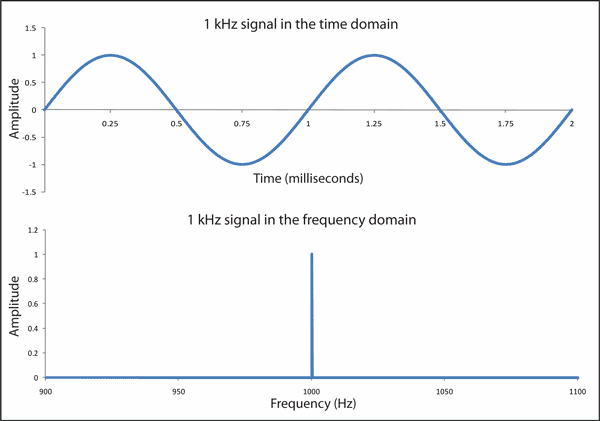
\includegraphics[width=\linewidth]{time_and_frequency_domain}
	\caption{: time domain vs frequency domain}
	\label{time_vs_freq}
\end{figure}
\\
So the Fourier transform is a tool that can make you go from the time domain \(f(t)\), to the frequency domain \(F(\omega)\). It is written as: \[F(\omega) = \int_{-\infty}^{\infty} f(t)e^{-j\omega t} dt \] There also is an inverse Fourier transform, logically this goes from the frequency domain to the time domain:\[f(t) = \frac{1}{2\pi} \int_{-\infty}^{\infty} F(\omega)e^{j\omega t} d\omega \] 

\newpage
But how to make sense of this formula? Lets split it up into several parts, starting with \(e^{-j\omega t} dt\). Euler's number to the power of  \(\sqrt{-1} = j = e^j\) moves around in a circle on the complex plane for every \(2\pi\) units. So if we want to describe a sine wave over time \((t)\) we can do \(e^{-j2\pi t}\), but we also need the frequency \((f)\) so that gives \(e^{-j2\pi f t}\) and since \(2 \pi f\) equals \(\omega\) we get \[e^{-j\omega t} \] Right so now you can plot this for a lot of frequencies (from \(-\infty\) to \(\infty\)) and you'd get a bunch of different positions on a circle in the complex plane. Now if you multiply this by your time domain function \(f(t)\) the positions in the circle will align just right with the frequencies that are most present in that function. That way the frequencies that are most present get magnified where frequencies that aren't present stay small. And that is how we get \[F(\omega) = \int_{-\infty}^{\infty} f(t)e^{-j\omega t} dt \]  

\subsection{Discrete Fourier Transform}

In the real world however you don't measure from negative infinity to infinity, since your data will always be over a finite time frame and your sensors won't be able to generate an infinite amount of samples. In the real world you will get a set of discrete points from when you begin plotting \((t_0)\) to the \(N^{th}\) sample \((t_{N-1})\) This is where the discrete Fourier transform (the DFT) comes in, it is described as \[X(k) = \sum_{n = 0}^{N -1} x[n]e^{\frac{-j 2 \pi k n}{N}}\]
Here it isn't an integral over infinity but a sum for all values of \((n = 0)\) to the total amount of samples \((N -1)\) Also in the exponential \(\frac{k}{N}\) now describes the frequency. But now it instead of any possible frequency we are limited to a set of frequencies which are defined by the sampling frequency, and the total amount of samples \((N)\). This is partly because of the Nyquist limit, which states that to accurately measure a frequency you need to sample at at least twice that frequency. And thus is is impossible to use any frequency higher than: $\frac{sample freqency}{2}$

The DFT is much more suitable for computation since it's a finite set of calculations. 

\subsection{The Fast Fourier Transform}
The computation time for computing a Fourier transform is proportional to the amount of samples (\(n\)) squared, \(n^2\) so naturally this gets slow rather fast the higher the number of samples gets. So in 1965 James Cooley and John Tukey developed the Fast Fourier transform (the FFT). With the FFT the computation time is proportional to \(\frac{n}{2}\) \(log_{2}\) \(n\) \cite{Sig} which is significantly faster.
We can see just how much faster it is if we divide \(n^2\) by \(\frac{n}{2}\) \(log_{2}\) \(n\) giving: \[y = \frac{2 n^2}{n log_{2} n}\] where y is the amount of times the FFT is faster and N being the nr of samples. When plotted it looks like this:
\begin{figure}[!ht]
	\centering
	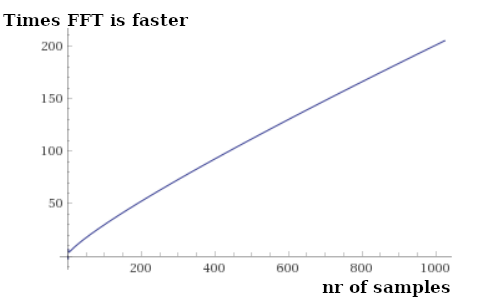
\includegraphics[width=\linewidth]{fft_tegen_ft}
	\caption{: Fourier vs Fast Fourier}
	\label{fourier_vs_fft}
\end{figure}\\
Here we can see that at 1024 samples the FFT is about two hundred times faster than a normal Fourier transform.
The FFT achieves this speed by recomposing larger point transformation out of several smaller point transformations. 

\section{How does the FFT work in two dimensions?} 
In radio astronomy the FFT is often used for image processing, images however aren't the one dimensional signals that we have been discussing so far. Images work in \textbf{two} dimensions, and these images too can be separated into a collection of sine and cosine waves. Here is an example of some two dimensional sine waves. 

\begin{figure}[!ht]
	\centering
	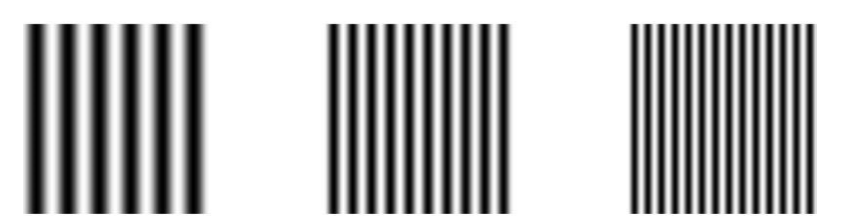
\includegraphics[width=\linewidth]{2d-sine}
	\caption{: Two dimensional sine waves }
	\label{2d_sine}
\end{figure}

Now the Fourier transform of these waves is surprisingly simple, a single or a few dot(s) in the right place can be used to describe these waves, as is shown here.

\begin{figure}[!ht]
	\centering
	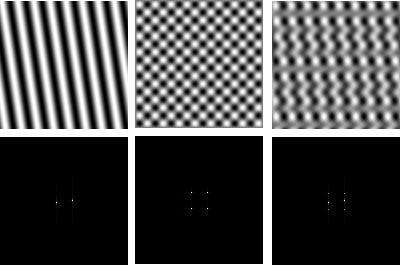
\includegraphics[scale=0.6]{sine_with_transform}
	\caption{: Two dimensional sine waves with their Fourier transforms}
	\label{2d_sine_with_transform}
\end{figure} 

Here you can already see that as more dots are added in the frequency domain the two dimensional image gets more complex. And thus you can imagine that any Two dimensional picture can be represented using a matrix of dots in the frequency domain. If colour pictures want to be achieved you will need three of these grey value matrices. One for red, one for green and one for blue when those are put on top of each other a colour picture is made.\par
In radio astronomy it works the other way around. Instead of having an image which has to be translated to the frequency domain, the array of radio telescopes receives their information in the frequency domain and will have to get it back into the time domain to get a coherent image. To achieve this a reverse FFT will have to be applied on the data. This image from radioastronomydm\cite{interferometry} shows it quite well (transformation goes from right to left): 

\begin{figure}[!ht]
	\centering
	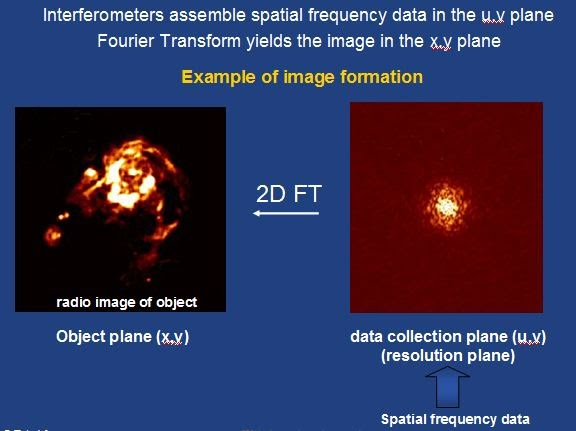
\includegraphics[width=\linewidth]{example_fft}
	\caption{: Fourier transform use in radio astronomy}
	\label{FFT use in radio astronomy}
\end{figure} 

But how exactly does it do this, well that is actually quite simple. First you look at the image as a matrix of values, then you apply a Fourier transformation over the rows, and then over the columns. And that's it, now for the inverse Fourier transform you will have to apply it over the columns first and then end with the rows to get the original image.     

\section{How are we planning to set up a test platform}

We want to simulate a multi processor system that preforms a two dimensional inverse FFT on an image. We want to measure the effect of adding and subtracting processors on calculation time and how that affects power consumption. \par 

To simulate the multi processor system we will use a stack of raspberry pi's. For the measuring of the power consumption we have developed hardware, and data logging software. These will be discussed in chapter \textbf{(!!!! placeholder for chapter on hardware and logging software !!!!)} 

For the algorithm we want the stack to be able to compute a two dimensional FFT and, the inverse two dimensional FFT.\\ To test if it works we will feed the program an image of which we know what the outcome should be. Like shown in the examples from figure \ref{2d_sine_with_transform}. Then if it passes that test we will feed that image back into the stack to see if it's inverse FFT transformation brings it back to the original image. If so, the program works.\\


as illustrated here (Illustration image of test here) 
\\

Now we also want to know what the influence of multi processing is on power consumption and computation speed, so we will have to design the algorithm in a way that enables us to add and subtract processors and it should still be able to run. That way we can run the algorithm on a single to \(n\) amount of processors, and measure the effects. 






\bibliographystyle{ieeetr}
\bibliography{bibliography.bib}

\end{document}